\documentclass{standalone}
\usepackage{picture,color}
\usepackage{graphicx}
\graphicspath{{./scan_1_raw/}}
\setlength{\unitlength}{1in}
\renewcommand{\rmdefault}{phv} % Arial
\renewcommand{\sfdefault}{phv} % Arial

\begin{document}
\begin{picture}(7.35, 7.94)(-0.09,-9.38)
%PNR image  
\put(-0.08, -7.8){\large\textbf{C}}
\put(.0, -9.235){\rotatebox{90}{\large residual}}
\put(.0, -8.5){\rotatebox{90}{\large raw data}}
\put(0.15, -8.55){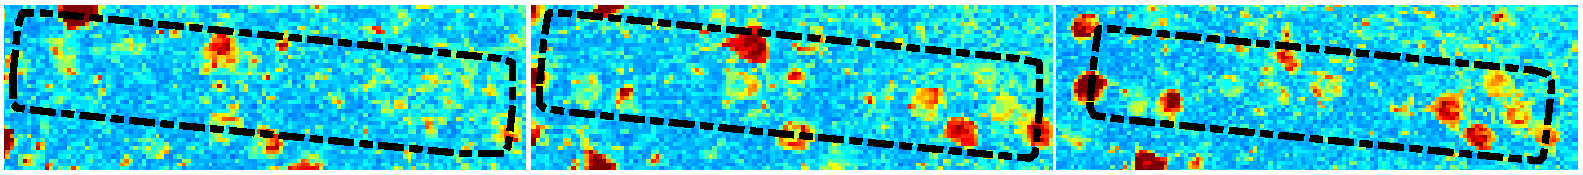
\includegraphics[height=0.76in]{scan_1_raw/pnr_before_horizontal.pdf}}
\put(0.15, -9.33){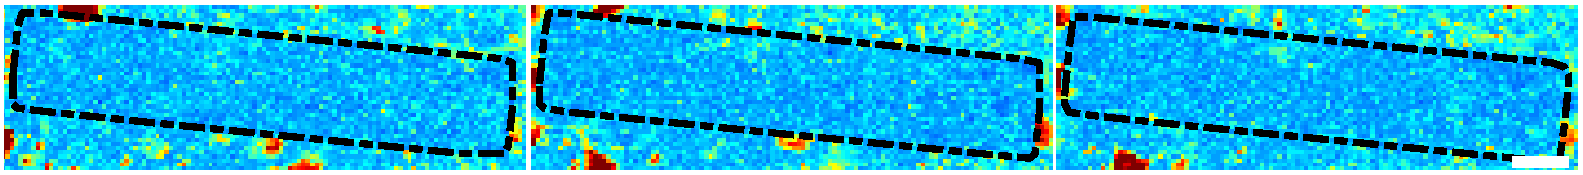
\includegraphics[height=0.76in]{pnr_after_horizontal.pdf}}
\put(7.03, -9.36){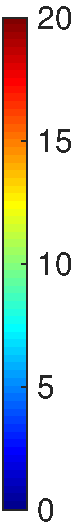
\includegraphics[height=1.61in]{pnr_colorbar.pdf}}
\put(1.05, -7.75){\large slice 1}
\put(3.35, -7.75){\large slice 2}
\put(5.65, -7.75){\large slice 3}

% example neurons 
\put(-0.08, -1.59){\large\textbf{A}}
\put(0.02, -4.9){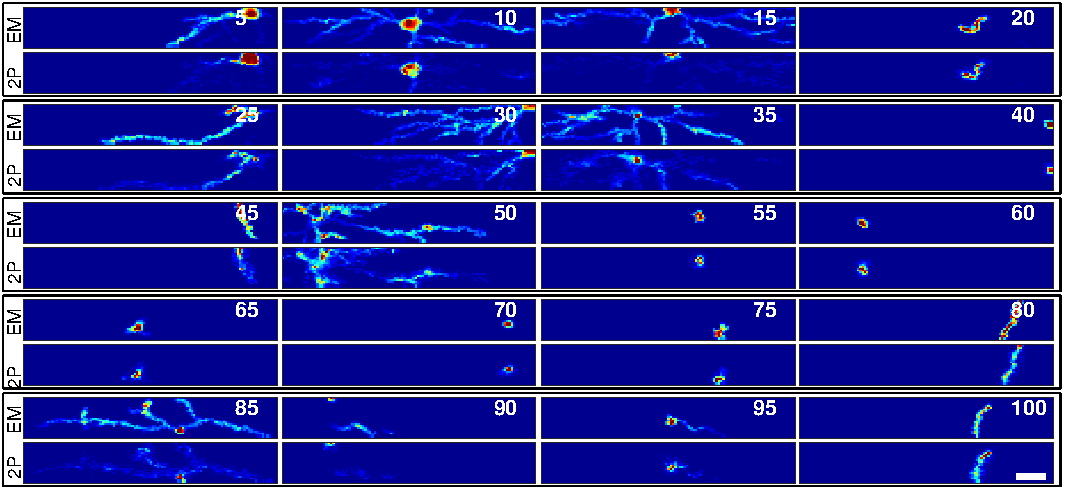
\includegraphics[height=3.31in]{fig_example_one_scan_a.pdf}}


% insert temporal trace 
\put(-0.1, -7.65){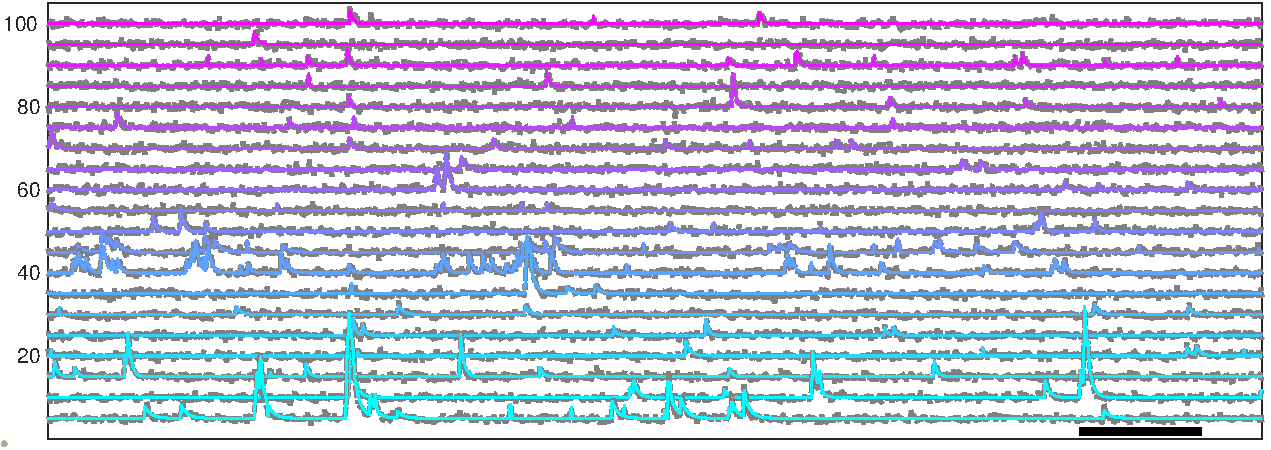
\includegraphics[height=2.615in]{temporal_examples.pdf}}
% \put(3.34, -5.65){Example temporal traces}
\put(-0.08, -5.05){\large\textbf{B}}

\end{picture}
\end{document}\grid
